\Echapter{DTI Distortion Correction with Conditionals}{Daniel J. Peterson}{djpeters@uw.edu}
\label{chap:dti}

In this example, we will use a Makefile to apply the appropriate
distortion correction procedure automatically, using conditionals. The
code for this example may be found in
\texttt{dti_suceptibility_correction/subjects}, in Makefiles in the
directories \texttt{fugue_DTI}, \texttt{topup_DTI}, and
\texttt{toy_test} as described below.

First, a bit of background: The most common way to acquire a series of
MRI images as quickly as possible is to use what is called an
``echo-planar imaging readout,'' or ``EPI.'' A drawback that comes
with this rapid acquisition is that EPI images are prone to
distortions due to an uneven magnetic field. Sometimes these
distortions are called ``susceptibility-induced distortions,'' because
it is the differing magnetic susceptibility of tissue, bone, and air
that causes the magnetic field to be uneven. Fortunately, because these
distortions are constant and predictable within an imaging session,
they can be undone.

We will consider two ways of undoing these distortions, each requiring
at least one extra image to be acquired. The first method is to
acquire an image of the uneven magnetic field, called a ``fieldmap.''
This image contains a map of the deviation from the main magnetic
field, in radians/sec (the resonance frequency of the water protons is
directly proportional to the strength of the magnetic field as per the
Larmor equation: $\omega=\gamma B _{0}$). To do this we will use a
tool called \texttt{fugue}, which is distributed as part of
FSL. \texttt{fugue} will convert this fieldmap into a nonlinear warp,
and then we can apply that warp to undo the susceptibility-induced
distortions. The other method is to acquire an additional image with
the EPI readout going in the other direction, meaning that the
direction of the susceptibility-induced distortion will be
reversed. We can then use a tool called \texttt{topup} (also from
FSL), that will warp two images with opposite distortions towards each
other, until they meet in the middle. We can then apply this computed
warp to the rest of our data.


These are two different procedures that require different sets of
files (an acquisition parameters file for \texttt{topup} and a
fieldmap for \texttt{fugue}), but can be part of an otherwise similar
pipeline. We can use \maken{} to sense which procedure to use based on
what files are present, and assemble the appropriate prerequisites.


To help understand the behavior of \maken{}, we have created an
example of a ``toy'' makefile, which does not call any real programs,
and can operate on empty ``dummy'' files. When debugging and
developing makefiles it can be useful to write such simplified
makefiles, and run them with \maken{}~\texttt{-n}. The code for this
Makefile is in \texttt{dti_suceptibility_correction/subjects/toy_test/Makefile}.


\begin{lstlisting}
	%*\lnote*SDC_METHOD = $(shell if [ -f fieldmap ] ; then echo FUGUE; \
                    elif [ -f acqparams ] ; then echo TOPUP; \
                    else echo FALSE ; fi)

	motion_corrected_dataset: raw_diffusion_dataset
	    toy_eddy.sh raw_diffusion_dataset

	topup_result: raw_diffusion_dataset acqparams
	    toy_topup.sh raw_diffusion_dataset acqparams

	%*\lnote*ifeq ($(SDC_METHOD),TOPUP)

	fully_corrected_diffusion_dataset: raw_diffusion_dataset topup_result
	    toy_eddy.sh raw_diffusion_dataset topup_result

	else ifeq ($(SDC_METHOD),FUGUE)
	fully_corrected_diffusion_dataset: motion_corrected_dataset fieldmap
	    toy_fugue.sh motion_corrected_dataset fieldmap
	    
	else
	%*\lnote*$(error ERROR: neither fieldmap for FUGUE \
	               nor acquisition parameter file for TOPUP were found)
	endif

	tensor: fully_corrected_diffusion_dataset
	    toy_solve_tensor.sh fully_corrected_diffusion_dataset

\end{lstlisting}


\lnum{1}If there is a file called \texttt{fieldmap} in the working directory we want to use \texttt{fugue}, and if \texttt{acqparams} exists instead, we want to use \texttt{topup}.

\lnum{2}When \maken{} runs, it will insert a different recipe into the set of rules depending on the value of \texttt{SDC_METHOD}. The conditional block extends until \texttt{endif}. The \texttt{else ifeq} statement in the middle is part of the same conditional block (i.e. you only need one \texttt{endif}).

\lnum{3}It's always a good idea to halt and raise an error if none of the expected conditions are met. \break

If we run this makefile to build the \texttt{tensor} target (using the \texttt{-n} flag) in a directory that contains both \texttt{raw_diffusion_dataset} and \texttt{fieldmap}, the result looks like this:

\bashcmd{make -n tensor \\toy_eddy.sh raw_diffusion_dataset \\toy_fugue.sh motion_corrected_dataset fieldmap \\toy_solve_tensor.sh fully_corrected_diffusion_dataset}

However, if both \texttt{raw_diffusion_dataset} and \texttt{acqparams} (and not \texttt{fieldmap}) are in the directory, we see:

\bashcmd{make -n tensor \\toy_topup.sh raw_diffusion_dataset acqparams \\toy_eddy.sh raw_diffusion_dataset topup_result \\toy_solve_tensory.sh fully_corrected_diffusion_dataset}

\autoref{toy-example} is a flowchart of the toy makefile.

\begin{figure}
	\begin{center}  % not necessary, but usually preferred.
		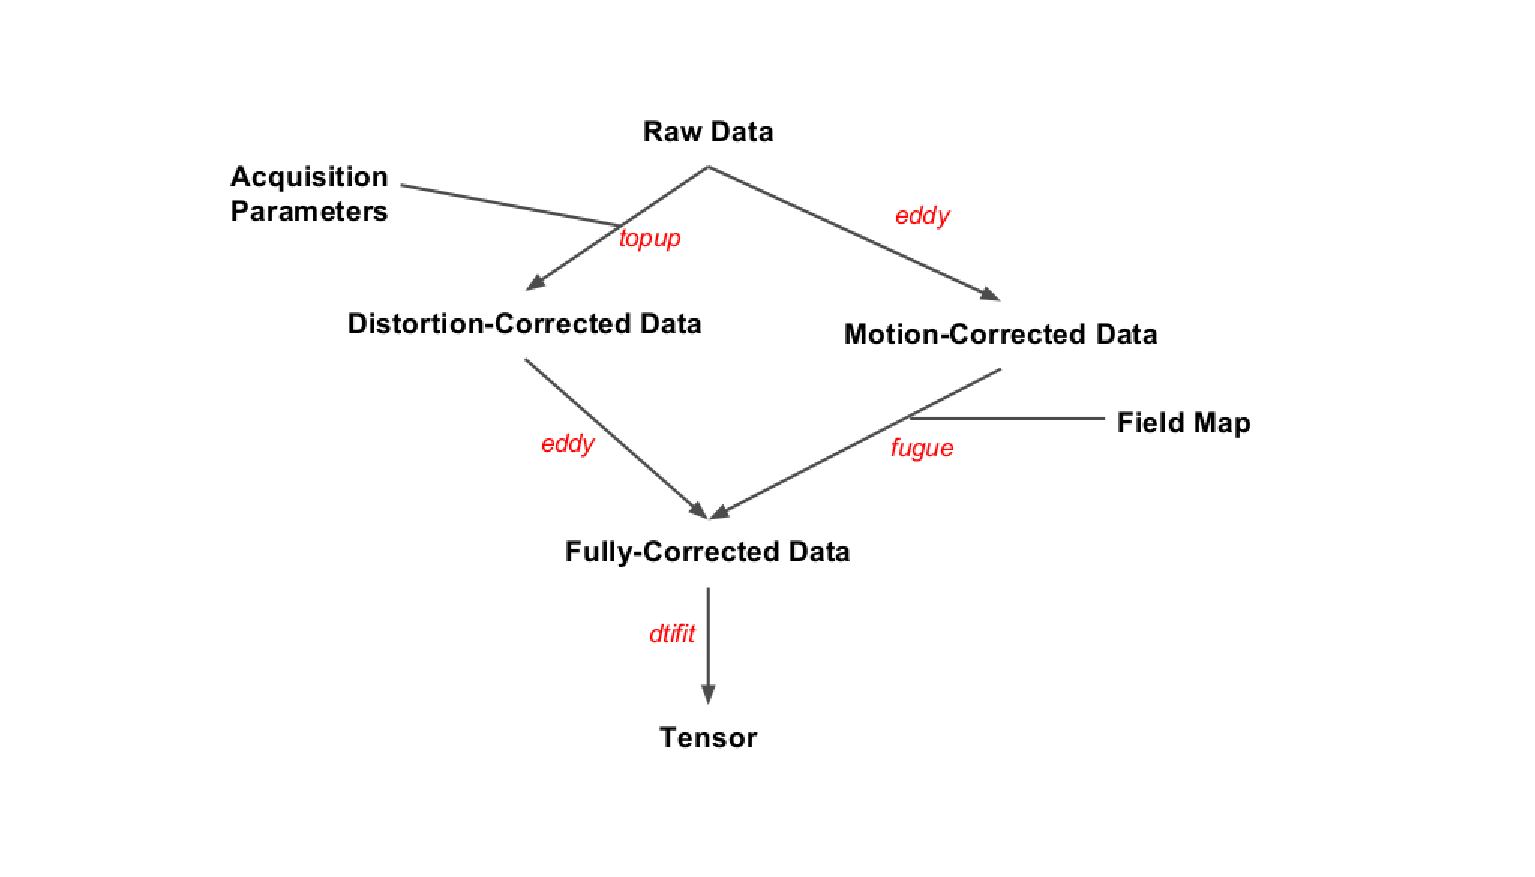
\includegraphics[width=\textwidth]{../images/distcorr-flowchart.eps}
	\end{center}
	\caption{Flowchart of the Toy Makefile}
	\label{toy-example}
\end{figure}


If we were to implement this process in a \bashn{} script, the earlier
``upstream'' processes would need to be part of the conditional
block. An advantage of using \maken{} for workflows is that
\emph{only} the part that causes the ``split'' in the branching logic
needs to be surrounded by the if-then-else-end logic. Also note that
if we were using \texttt{topup} with a fieldmap, but for some reason
we wanted to do just the motion correction (like for QC, or for
debugging purposes), that unused ``branch'' of the makefile would be
available with a simple \texttt{make motion_corrected_dataset}
command. \newpage


Here's the full Makefile, located in
\texttt{dti_suceptibility_correction/subjects/fugue_DTI} and
\texttt{dti_suceptibility_correction/subjects/topup_DTI}. You can see
each of these files is in fact a symbolic link to the same file, located in
\texttt{dti_suceptibility_correction/lib/diffusion.Makefile}.

\setcounter{codehighlight}{0}
\begin{lstlisting}
	ifeq "$(origin MAKEPIPELINES)" "undefined"
	MAKEPIPELINES=/project_space/makepipelines
	endif

	PROJECT_DIR=$(MAKEPIPELINES)/dti_suceptibility_correction

	SDC_METHOD = $(shell if [ -f fieldmap.nii.gz ] ; then echo FUGUE; \
	                    elif [ -f acqparams.txt ] ; then echo TOPUP; \
	                    else echo FALSE ; fi)


	%*\lnote*NUM_DIFFUSION_VOLS =$(shell fslval raw_diffusion.nii.gz dim4 | tr -d '\040\011\012\015')


	%*\lnote*EDDY_ITERATIONS = 1
	TOPUP_MODE=fast
	ECHO_SPACING =.00072
	UNWARP_DIRECTION=y-

	.PHONY: clean tensor

	%*\lnote*mec_diffusion.nii.gz: raw_diffusion.nii.gz bval bvec brain_mask.nii.gz
		echo "0 1 0 0.072" > temp_acqparams.txt ;\
		for i in `seq 1 $(NUM_DIFFUSION_VOLS)`; do echo 1 >> temp_index.txt ; done ;\
		eddy --imain=raw_diffusion.nii.gz --mask=brain_mask.nii.gz \
			--index=temp_index.txt --acqp=temp_acqparams.txt --bvecs=bvec \
			--bvals=bval --out=mec_diffusion --niter=$(EDDY_ITERATIONS) \
			--verbose  ;\
		rm temp_acqparams.txt temp_index.txt

	%*\lnote*topup_results_movpar.txt: raw_diffusion.nii.gz acqparams.txt
		fslroi raw_diffusion.nii.gz S0_images.nii.gz 0 2 ;\
		topup --imain=S0_images --datain=acqparams.txt \
			--config=$(PROJECT_DIR)/lib/b02b0_$(TOPUP_MODE).cnf \
			--out=topup_results --fout=field_est --iout=unwarped_S0_images \
			--verbose

	ifeq ($(SDC_METHOD),TOPUP)
	sdc_mec_diffusion.nii.gz: raw_diffusion.nii.gz topup_results_movpar.txt index.txt
		eddy --imain=raw_diffusion.nii.gz --mask=brain_mask --acqp=acqparams.txt \
			--index=index.txt --bvecs=bvec --bvals=bval \
			--topup=topup_results \
			--out=sdc_mec_diffusion.nii.gz --niter=$(EDDY_ITERATIONS) \
			--verbose
		
	else ifeq ($(SDC_METHOD),FUGUE)
	sdc_mec_diffusion.nii.gz: mec_diffusion.nii.gz fieldmap.nii.gz
		fugue --loadfmap=fieldmap.nii.gz --dwell=$(ECHO_SPACING) \
			-i mec_diffusion.nii.gz -u sdc_mec_diffusion.nii.gz \
			--unwarpdir=$(UNWARP_DIRECTION) -v
	else
	$(error ERROR: neither fieldmap for FUGUE nor acquisition parameter file for TOPUP were found)
	endif

	tensor: sdc_mec_diffusion.nii.gz brain_mask.nii.gz bvec bval
		dtifit -k sdc_mec_diffusion.nii.gz -r bvec -b bval -m brain_mask -o dti

	clean:
		rm -f dti_* sdc_mec_diffusion.* mec_diffusion.* S0_images* \
		field_est.nii.gz topup_results* unwarped_S0_images.nii.gz

\end{lstlisting}


\lnum{1}\texttt{fslval} returns a trailing space as part of its output, which we pipe to \texttt{tr} for deletion.

\lnum{2}The settings here are for a quick test run for demonstration
purposes. For more accurate (but slower) processing,
\texttt{TOPUP_MODE} can be changed to 'accurate', and
\texttt{EDDY_ITERATIONS} can be increased to 5. Placing the settings
clearly in the Makefile makes it easy to extract them for quality
assurance reports. 

\lnum{3}In addition to running \texttt{eddy}, this recipe creates a simple acquisition parameters file and a simple index file (\texttt{eddy} requires that you supply one). This tells \texttt{eddy} that all the images were acquired with the phase encoding along the same direction. These files are deleted afterwards.

\lnum{4}The first two images are assumed to be the two non-diffusion weighted images (i.e. the $S _{0}$ images), with the phase encoding along different directions.


There are a few more files and commands here than in the toy example,
but the basic structure is the same. It's still missing some elements
of a full-featured DTI preprocessing pipeline (for example, unwarping
the brain mask, coregistration of the fieldmap with the diffusion
data, and rotation of the b-vectors), but this example illustrates how
using conditional statements in makefiles can make them more robust
and versatile.

\vspace{\baselineskip}
\hrule
\vspace{\baselineskip}

More information about the options and the formats of the files
supplied to \texttt{eddy}, \texttt{topup}, and \texttt{fugue} is
available on the
\href{http://fsl.fmrib.ox.ac.uk/fsl/fslwiki/FslOverview}{FSL website}.





